\documentclass{standalone}
\usepackage{tikz}
\usepackage{ctex,siunitx}
\setCJKmainfont{Noto Serif CJK SC}
\usepackage{tkz-euclide}
\usepackage{amsmath}
\usepackage{wasysym}
\usetikzlibrary{patterns, calc}
\usetikzlibrary {decorations.pathmorphing, decorations.pathreplacing, decorations.shapes,}
\begin{document}
\small
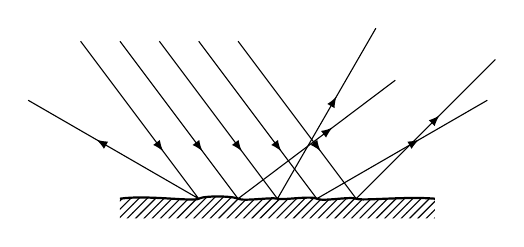
\begin{tikzpicture}[>=latex]
  \foreach \x/\y in {-1/150,-0.5/37,0/60,0.5/30,1/45}
  {
    \draw[postaction={decorate},decoration={markings,mark={between positions 0.35 and 0.9 step 0.45 with {\arrow{>}}}},line join=round] (\x-1.5,2.0)--(\x,0)--++(\y:2.5);
  }
  \fill [pattern=north east lines] (-2,-.25)--(-2.000, 0.000)..controls(-1.664, 0.050)and(-1.069,-0.040)..
  (-1.000, 0.000)..controls(-0.931, 0.040)and(-0.572, 0.036)..
  (-0.500, 0.000)..controls(-0.428,-0.036)and(-0.077, 0.021)..
  ( 0.000, 0.000)..controls( 0.077,-0.021)and( 0.431, 0.040)..
  ( 0.500, 0.000)..controls( 0.569,-0.040)and( 0.926, 0.031)..
  ( 1.000, 0.000)..controls( 1.074,-0.031)and( 1.629, 0.032)..( 2.000, 0.000) -- (2,-0.25)--cycle;
  \draw [thick](-2.000, 0.000)..controls(-1.664, 0.050)and(-1.069,-0.040)..
  (-1.000, 0.000)..controls(-0.931, 0.040)and(-0.572, 0.036)..
  (-0.500, 0.000)..controls(-0.428,-0.036)and(-0.077, 0.021)..
  ( 0.000, 0.000)..controls( 0.077,-0.021)and( 0.431, 0.040)..
  ( 0.500, 0.000)..controls( 0.569,-0.040)and( 0.926, 0.031)..
  ( 1.000, 0.000)..controls( 1.074,-0.031)and( 1.629, 0.032)..( 2.000, 0.000);
\end{tikzpicture}
\end{document}